\documentclass{report}



\usepackage{lipsum}
\usepackage{mwe}
\usepackage{enumerate}
\usepackage{booktabs}

\let\mc\multicolumn

\begin{document}

\begin{titlepage}
\begin{center}
\vspace*{1cm}

\textbf{Report Title}

\vspace{0.5cm}
 Bachelor title
            
\vspace{1.5cm}

\textbf{Author Name}

\vspace{1.5cm}
Alex Langhoff

	
       \vfill
            
A report presented for the degree of\\
Bachelor of computer sciene
            
       \vspace{0.8cm}
     
      
            
       Department Name\\
       University Name\\
       Country\\
       Date
            
   \end{center}
\end{titlepage}


\tableofcontents



\chapter{Alex lære lidt}
Alex er slet ikke så dum, han kan faktisk lære noget.

\section{One image, that is centered}
\lipsum[5]
\begin{figure}[h]
\centering
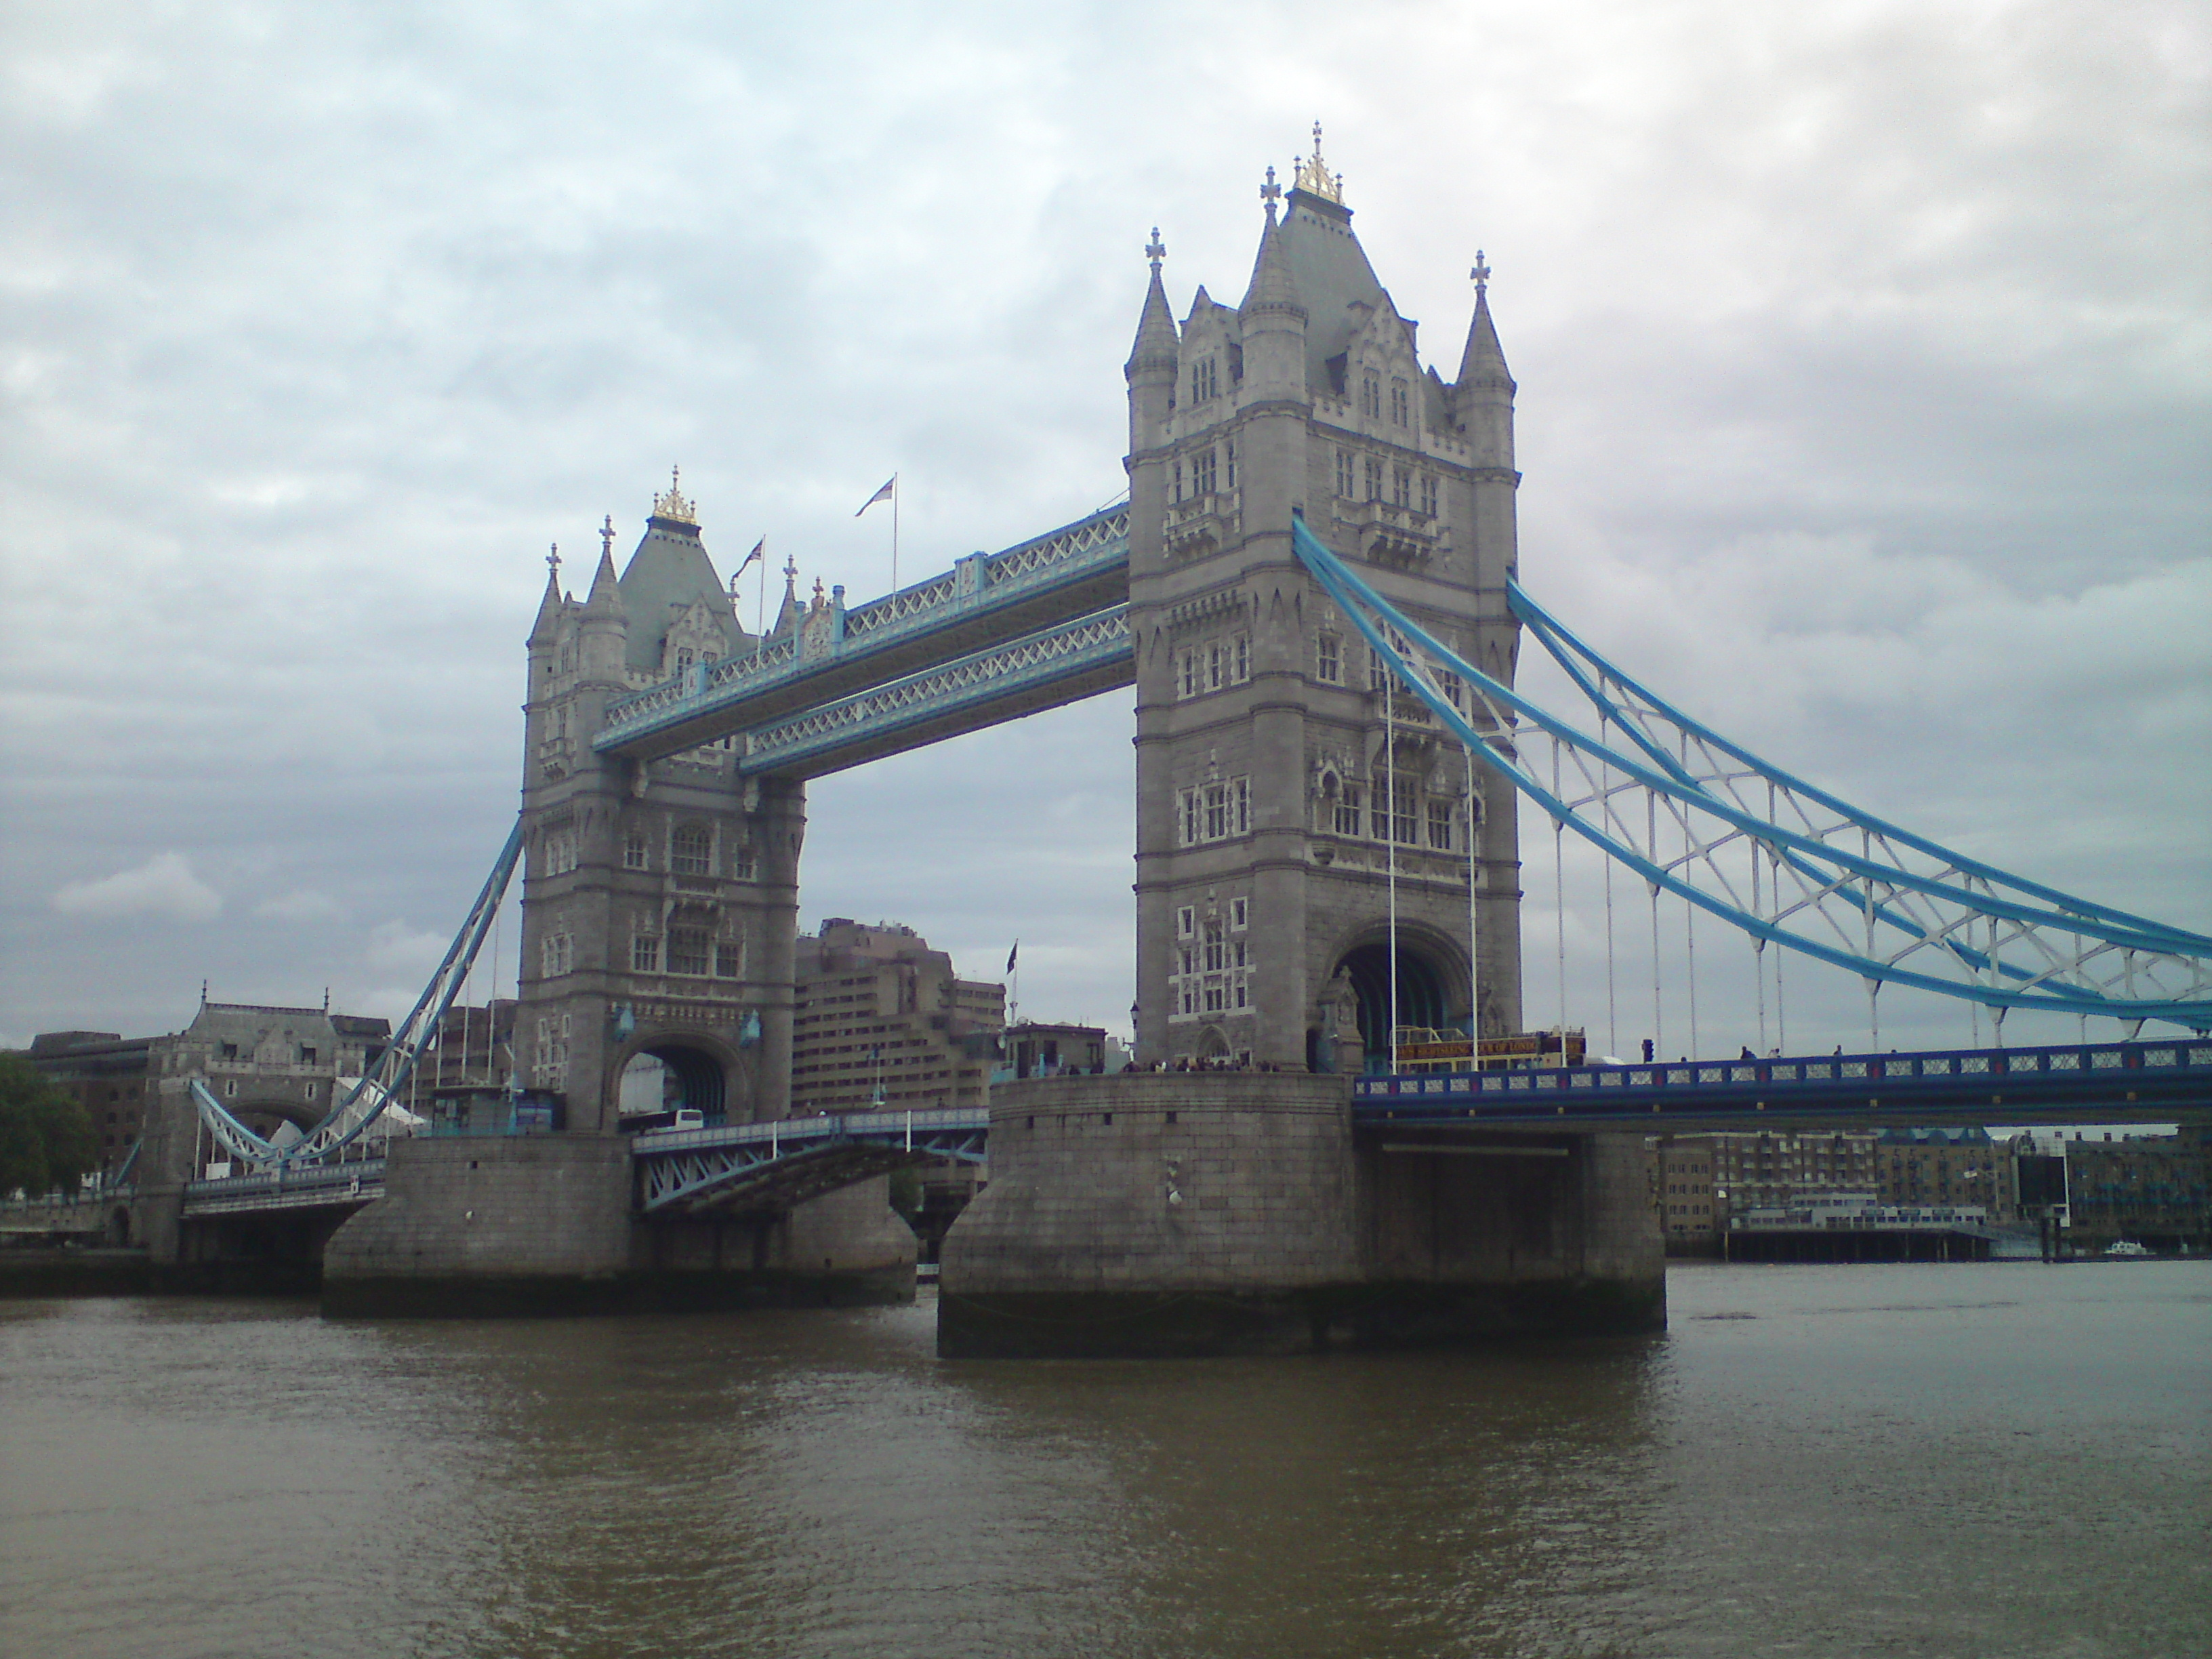
\includegraphics[scale=0.05]{D://Klasser//UFO//DSC00403.JPG}
\caption{En bro}\label{mylabel}
\end{figure}
\lipsum[3]
  
En bro, se figur ~\ref{mylabel} at page~\pageref{mylabel}



\section{Two images, that is centered}
\lipsum[5]
\begin{figure}[h]
\centering
\begin{minipage}{0.45\textwidth}
\centering
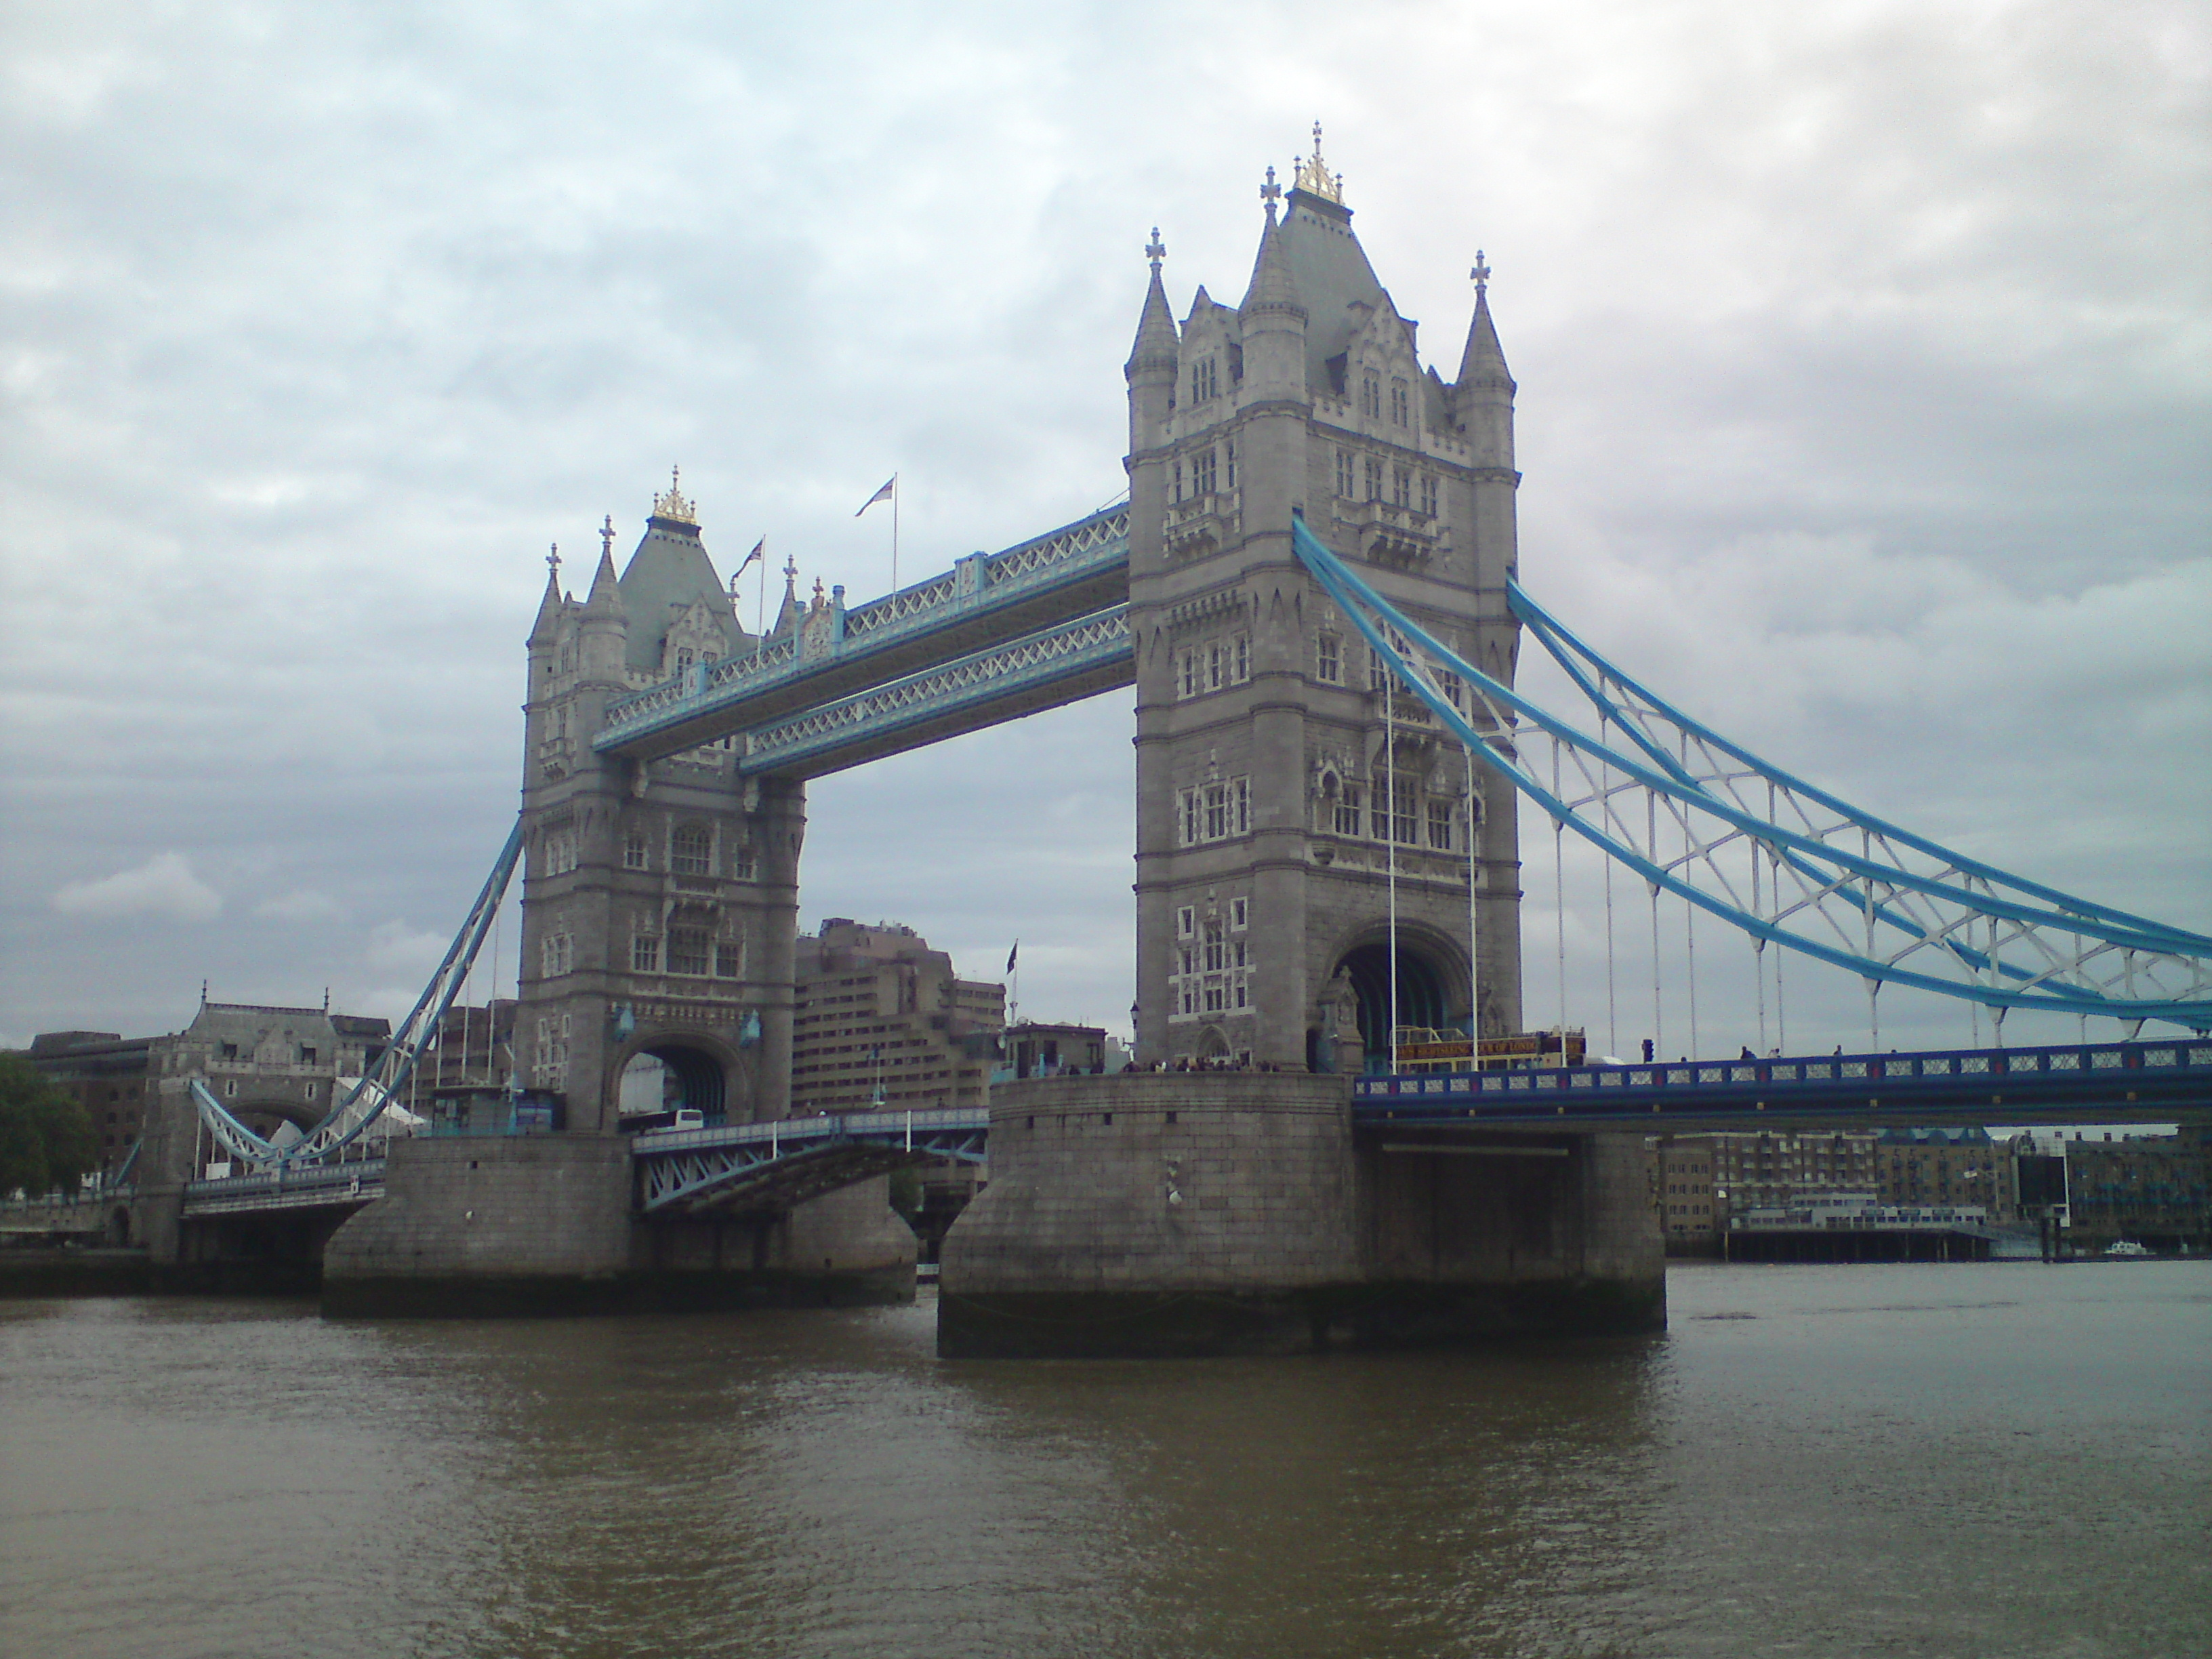
\includegraphics[scale=0.05]{D://Klasser//UFO//DSC00403.JPG}
\caption{En bro}
\end{minipage}\hfill
\begin{minipage}{0.45\textwidth}
\centering
\caption{En vigtig bro for England}
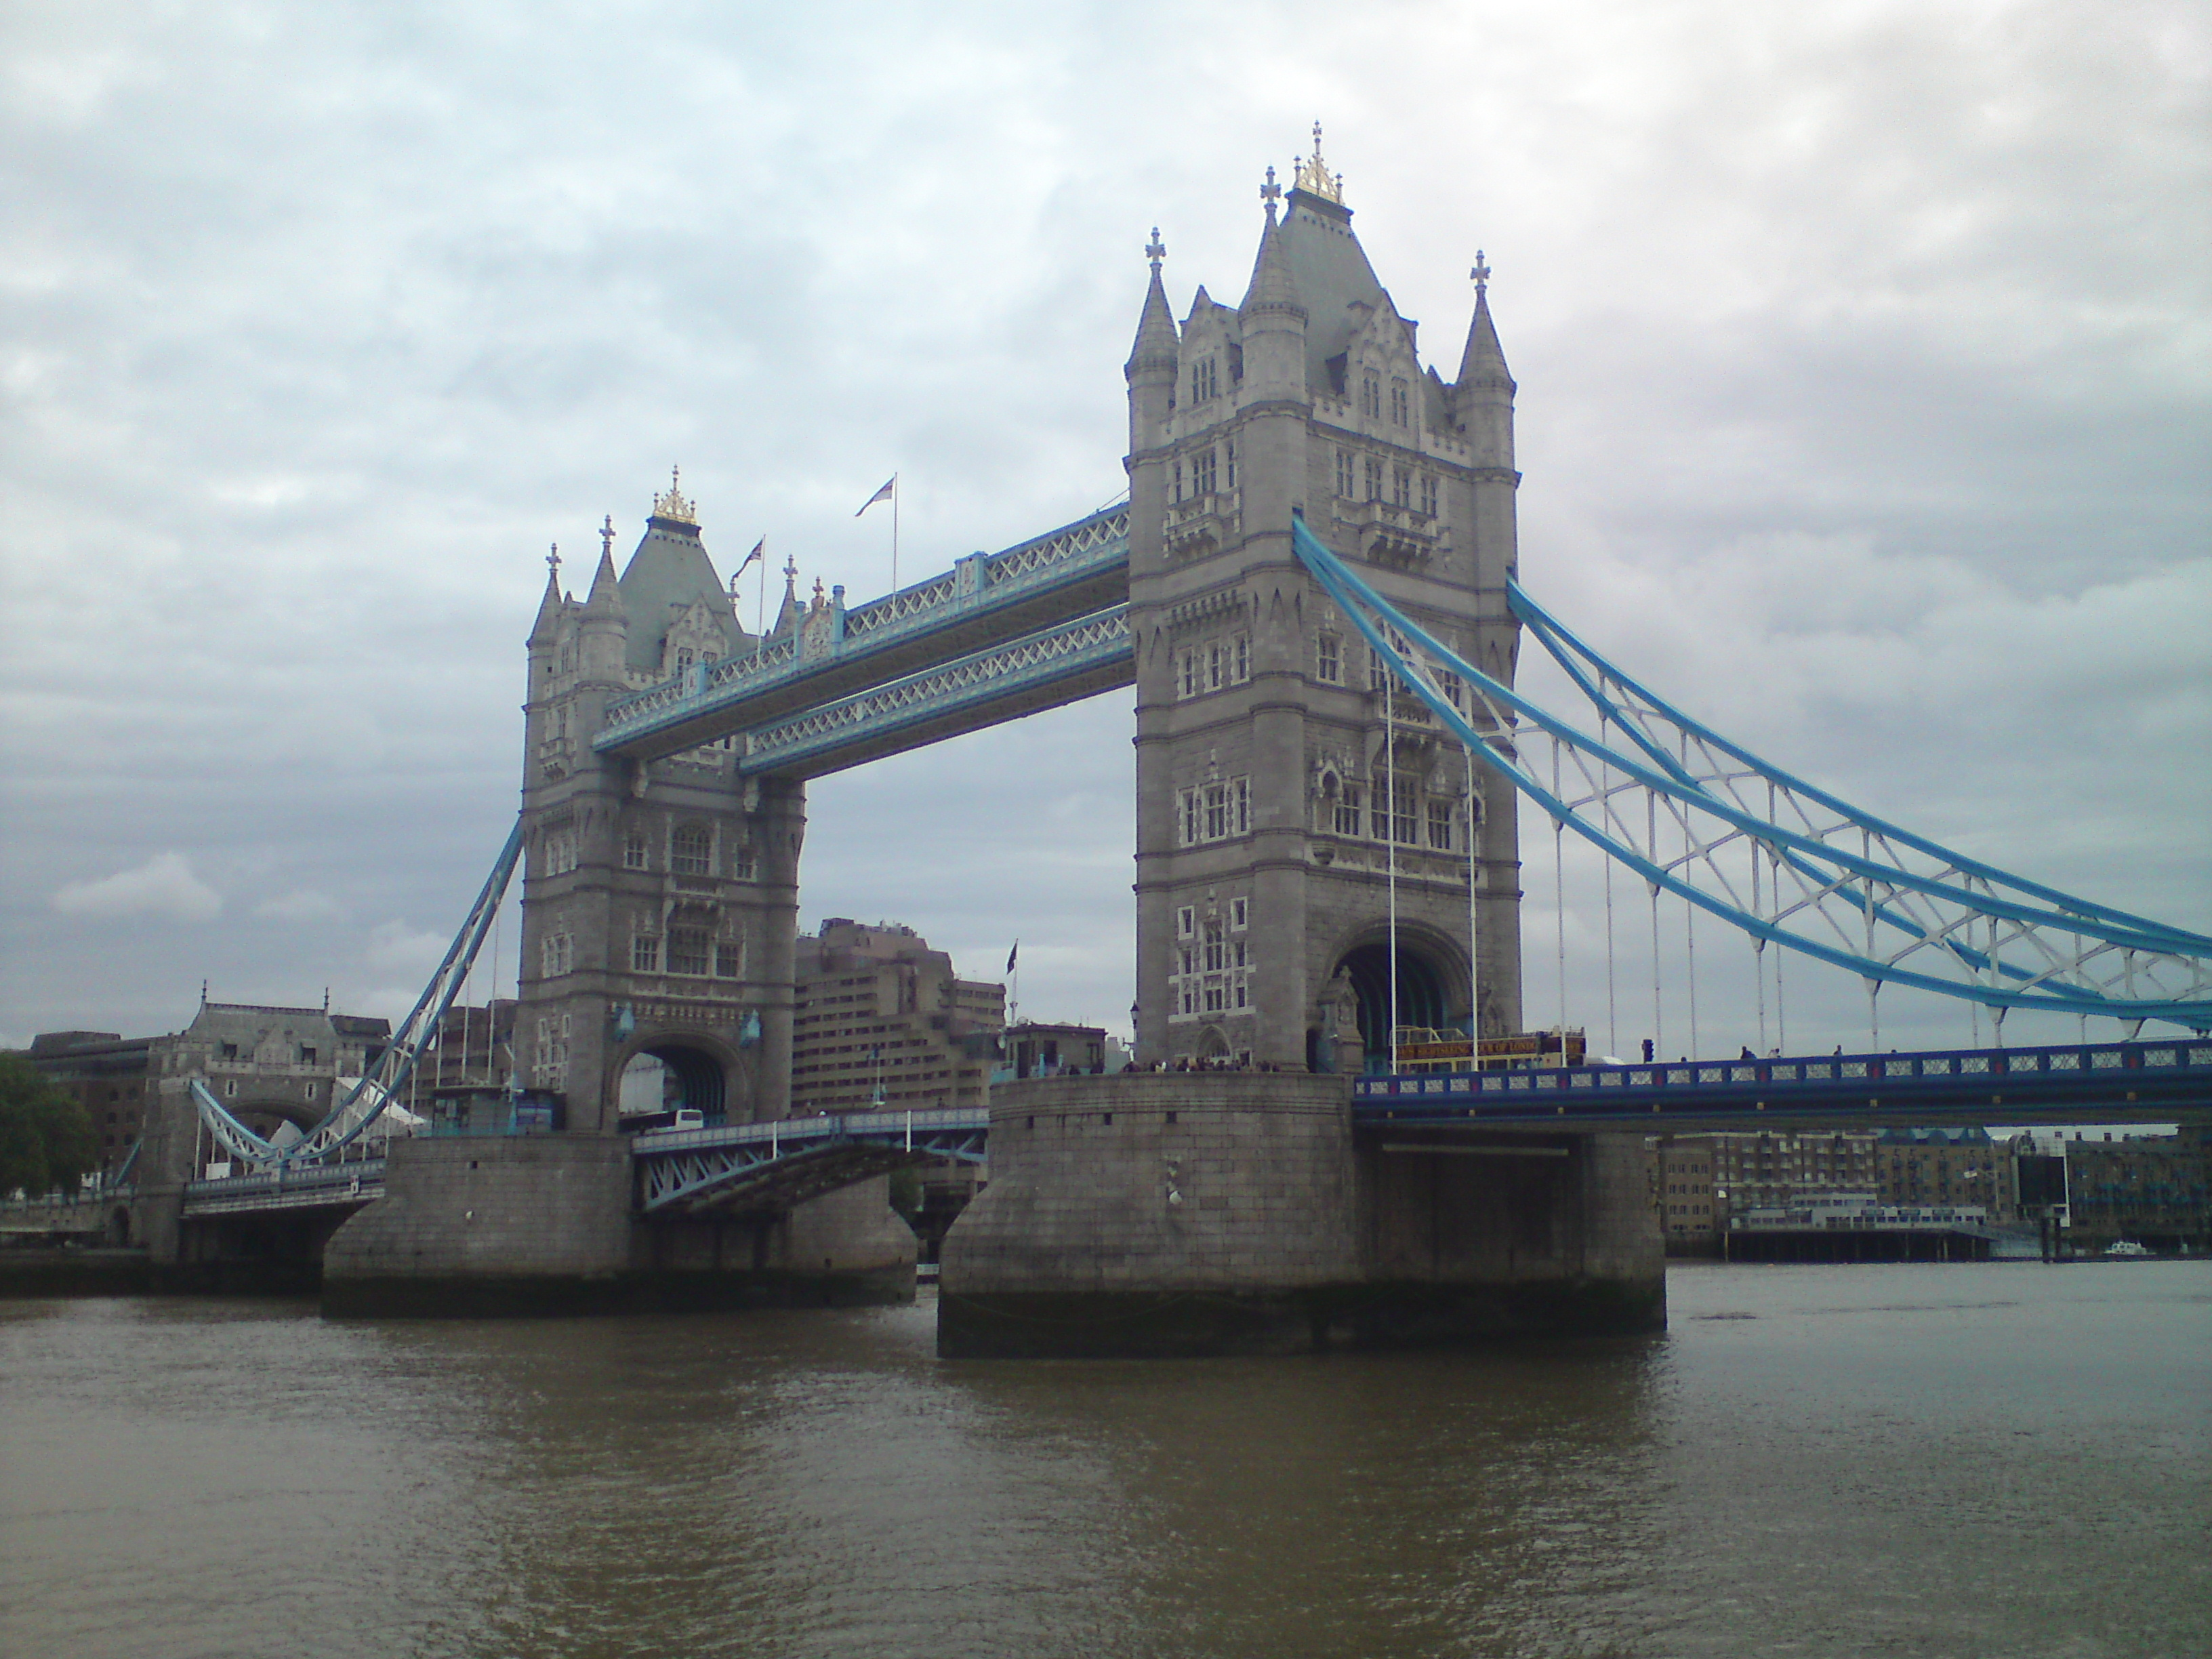
\includegraphics[scale=0.05]{D://Klasser//UFO//DSC00403.JPG}
\end{minipage}
\end{figure}
\lipsum[3]






\section{numbered section}
Hejsa, dette er min bog 
\today
Der står ikke så meget endnu, men det kommer...håber jeg.
\newpage
\section*{not numbered section}
Men meget kan ske. Mit Internet virker ikke i dag. Så jeg er stuck med Internet deling over min telefon...Det er langsomt.


\chapter{Bullet lists}

\section{Unordered lists}
\begin{itemize}
  \item The individual entries are indicated with a black dot, a so-called bullet.
  \item The text in the entries may be of any length.
\end{itemize}

\section{Ordered lists}
\begin{enumerate}
  \item The labels consists of sequential numbers.
  \item The numbers starts at 1 with every call to the enumerate environment.
\end{enumerate}

\section{list with other char}


\begin{enumerate}[-a]
  \item The individual entries are indicated with a black dot, a so-called bullet.
\item The individual entries are indicated with a black dot, a so-called bullet.
\end{enumerate}



\section{tables}
\begin{tabular}{r rrr rrr rr}
\toprule
 & \mc3c{Balanced Error} 
 & \mc3c{Area Under Curve}
 & \mc2c{Features} \\
 \cmidrule(r){2-4}
 \cmidrule{5-7} 
 \cmidrule(l){8-9}
  Data Set & Train &Valid &Test & Train &Valid & Test & \# & \% \\
\midrule
arcene&0.5000 &0.4886 &0.5006 & 0.5000 &0.5114 &0.4994 &10000 & 100.10\\
gisette&0.5000 &0.4886 &0.5006 & 0.5000 &0.5114 &0.4994 &10000 & 100.10\\
dexter&0.5000 &0.4886 &0.5006 & 0.5000 &0.5114 &0.4994 &10000 & 100.10\\ 
madelon&0.5000 &0.4886 &0.5006 & 0.5000 &0.5114 &0.4994 &10000 & 100.10\\
\bottomrule
\label{myrow}
\end{tabular}


  \section{test reference}
See table~\ref{myrow} on page~\pageref{myrow}

\section{cite}
Let's cite! The Einstein's journal paper \cite{einstein} and the Dirac's 
book \cite{dirac} are physics related items. 

\bibliographystyle{plain}

\bibliography{sample}




\end{document}